\documentclass[11pt,a4paper,titlepage]{article}
\usepackage[utf8]{inputenc}
\usepackage[english]{babel}
\usepackage{amsmath}
\usepackage{amsfonts}
\usepackage{amssymb}
\usepackage[left=2cm,right=2cm,top=2cm,bottom=2cm]{geometry}
\usepackage{hyperref}
\usepackage{graphicx}
\usepackage{caption}
\usepackage{subcaption}

\author{Adrian Wälchli}
\title{Bachelor Project Journal}

\begin{document}

\maketitle
\begin{abstract}
This report presents an overview of my bachelor thesis. We discuss several approaches to problems, experiments, ideas and evaluate results. This document will be extended over time as the project evolves.
\end{abstract}

\tableofcontents
\newpage

\section{Related work}
The basis of this project are the papers from \cite{WETZ_TOMO, WETZ_TENS}. Additional papers used for the work are: Light Field Rendering by Marc Levoy and Pat Hanrahan, Fourier Slice Photography by Ren Ng, Light Field Photography with a Hand-held Plenoptic Camera by Ren Ng et al. 

\section{Types of light fields} \label{sec:lftypes}
In this project, I encountered two types of 4D light fields that are captured using camera grids. The most common way of acquiring a light field is to capture a scene with a 2D-grid of cameras where the optical axes of the cameras are orthogonal to the camera grid. Since the look-at-point of each camera is different, this setup will result in a shift in the images formed on the sensors. An alternative way to capture the scene is to fix the look-at-point for every camera, preferably at the origin of the  scene. This is the type of light fields primarily used in the paper from \cite{WETZ_TOMO}. 
\\
In addition, the images can be optained using either perspective or orthographic projections. Sheared projections can also be used as mentioned in \cite[p.~4]{LEVO_LFREN}.

\begin{figure}
	\centering
	\begin{subfigure}[b]{0.4\textwidth}
 		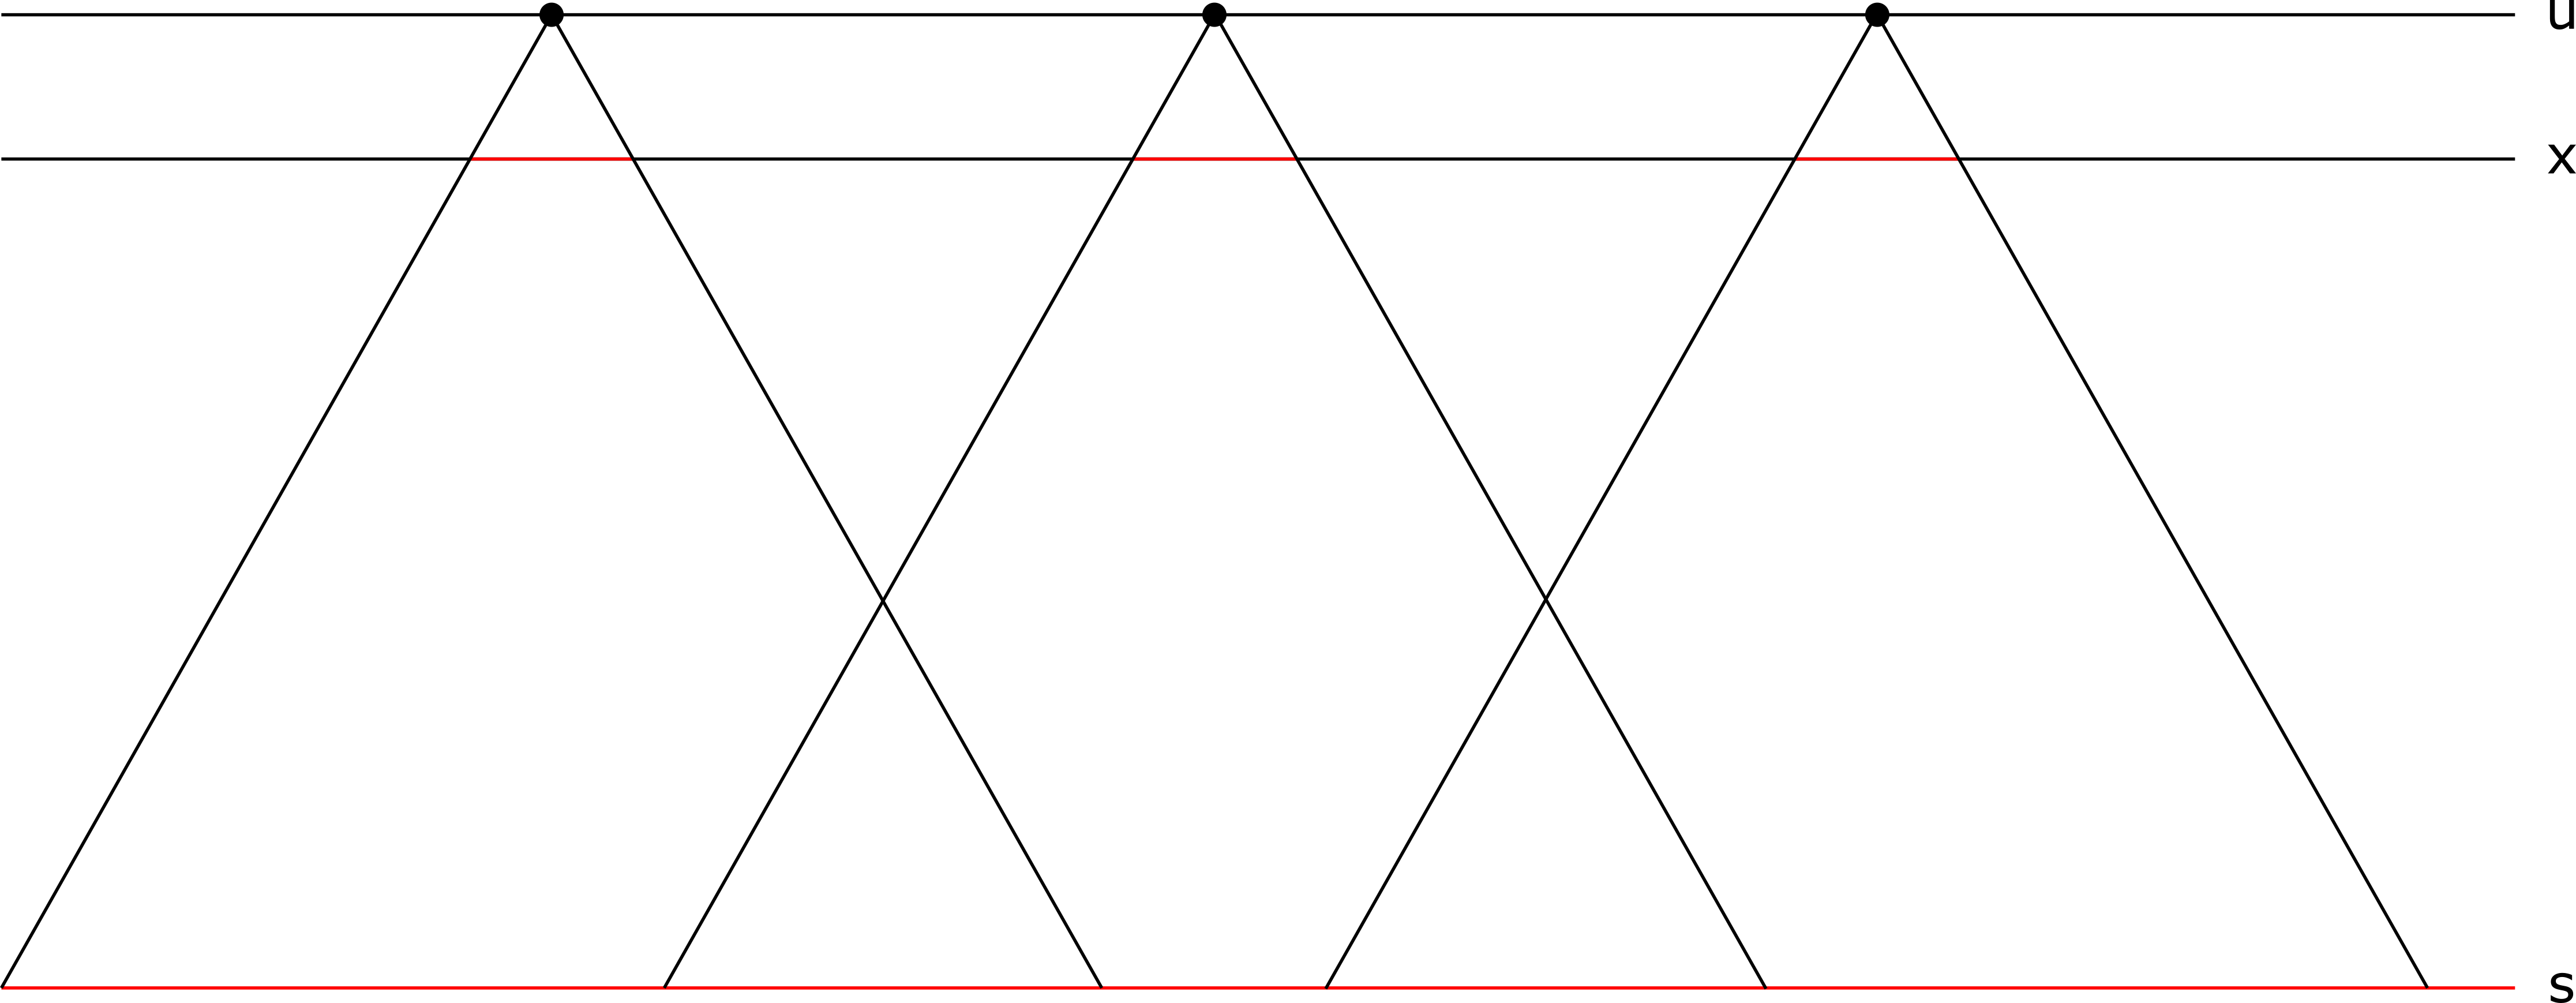
\includegraphics[width=\textwidth]{sketches/perspective_shifted_projections.png}
  		\caption{Perspective projections, images are shifted}
   		\label{fig:perspective_shifted_projections}
	\end{subfigure}%
	\qquad
	\begin{subfigure}[b]{0.4\textwidth}
		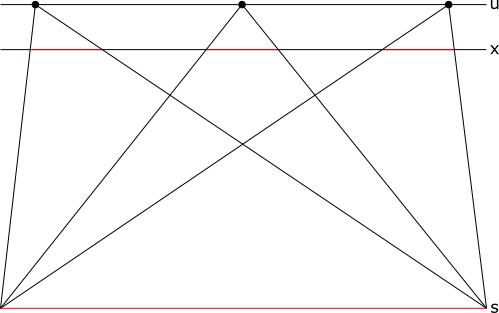
\includegraphics[width=0.65\textwidth]{sketches/sheared_projections.png}
		\caption{Sheared Projections, cameras have a common image plane}
		\label{fig:sheared_projections}
	\end{subfigure}
	\caption{Different methods to capture a lightfield}\label{fig:animals}
\end{figure}

\section{Notation}

The two-plane representation is used to describe a 4D-light field $l\left( u, v, s, t \right)$, where $\left( u, v \right)$ is the coordinate for the camera plane and $\left( s, t \right)$ for the focal plane. 

\begin{center}
	\begin{tabular}{|l|l|}
	
		\hline
		Symbol 	& Meaning \\
		\hline 
		$d_c$ 	& Distance between two cameras \\ 
		\hline 
		$d_s$ 	& Distance between image plane and center of projection \\ 
		\hline 
		$z$ 	& Distance between the camera plane and the scene origin \\ 
		\hline
		$u_j$	& Position of camera $j$ \\
		\hline
		$x_j^i$ & Position of pixel $j$ on the image plane of camera $i$ \\
		\hline
		$s_j^i$ & Position of pixel $j$ on layer $i$ \\ 
		\hline 
		$d_L$ 	& Distance between two layers \\ 
		\hline 

	\end{tabular} 
\end{center}

\section{A first implementation for orthographic projections}	\label{sec:first_implementation}
In a first step, I (re-)implemented the tomographic light field synthesis for layered 3D-displays in MATLAB, based on the theory in \cite{WETZ_TOMO} and their publicly available MATLAB code. The core problem to solve is:

\begin{equation} \label{eq:core_problem}
	\begin{aligned}
		& \underset{x}{\text{argmin}} & & \| Px - \bar{l} \| \\
		& \text{subject to} & & 0 \leq x \leq 1
	\end{aligned}
\end{equation}

\begin{figure}[h]
	\centering
	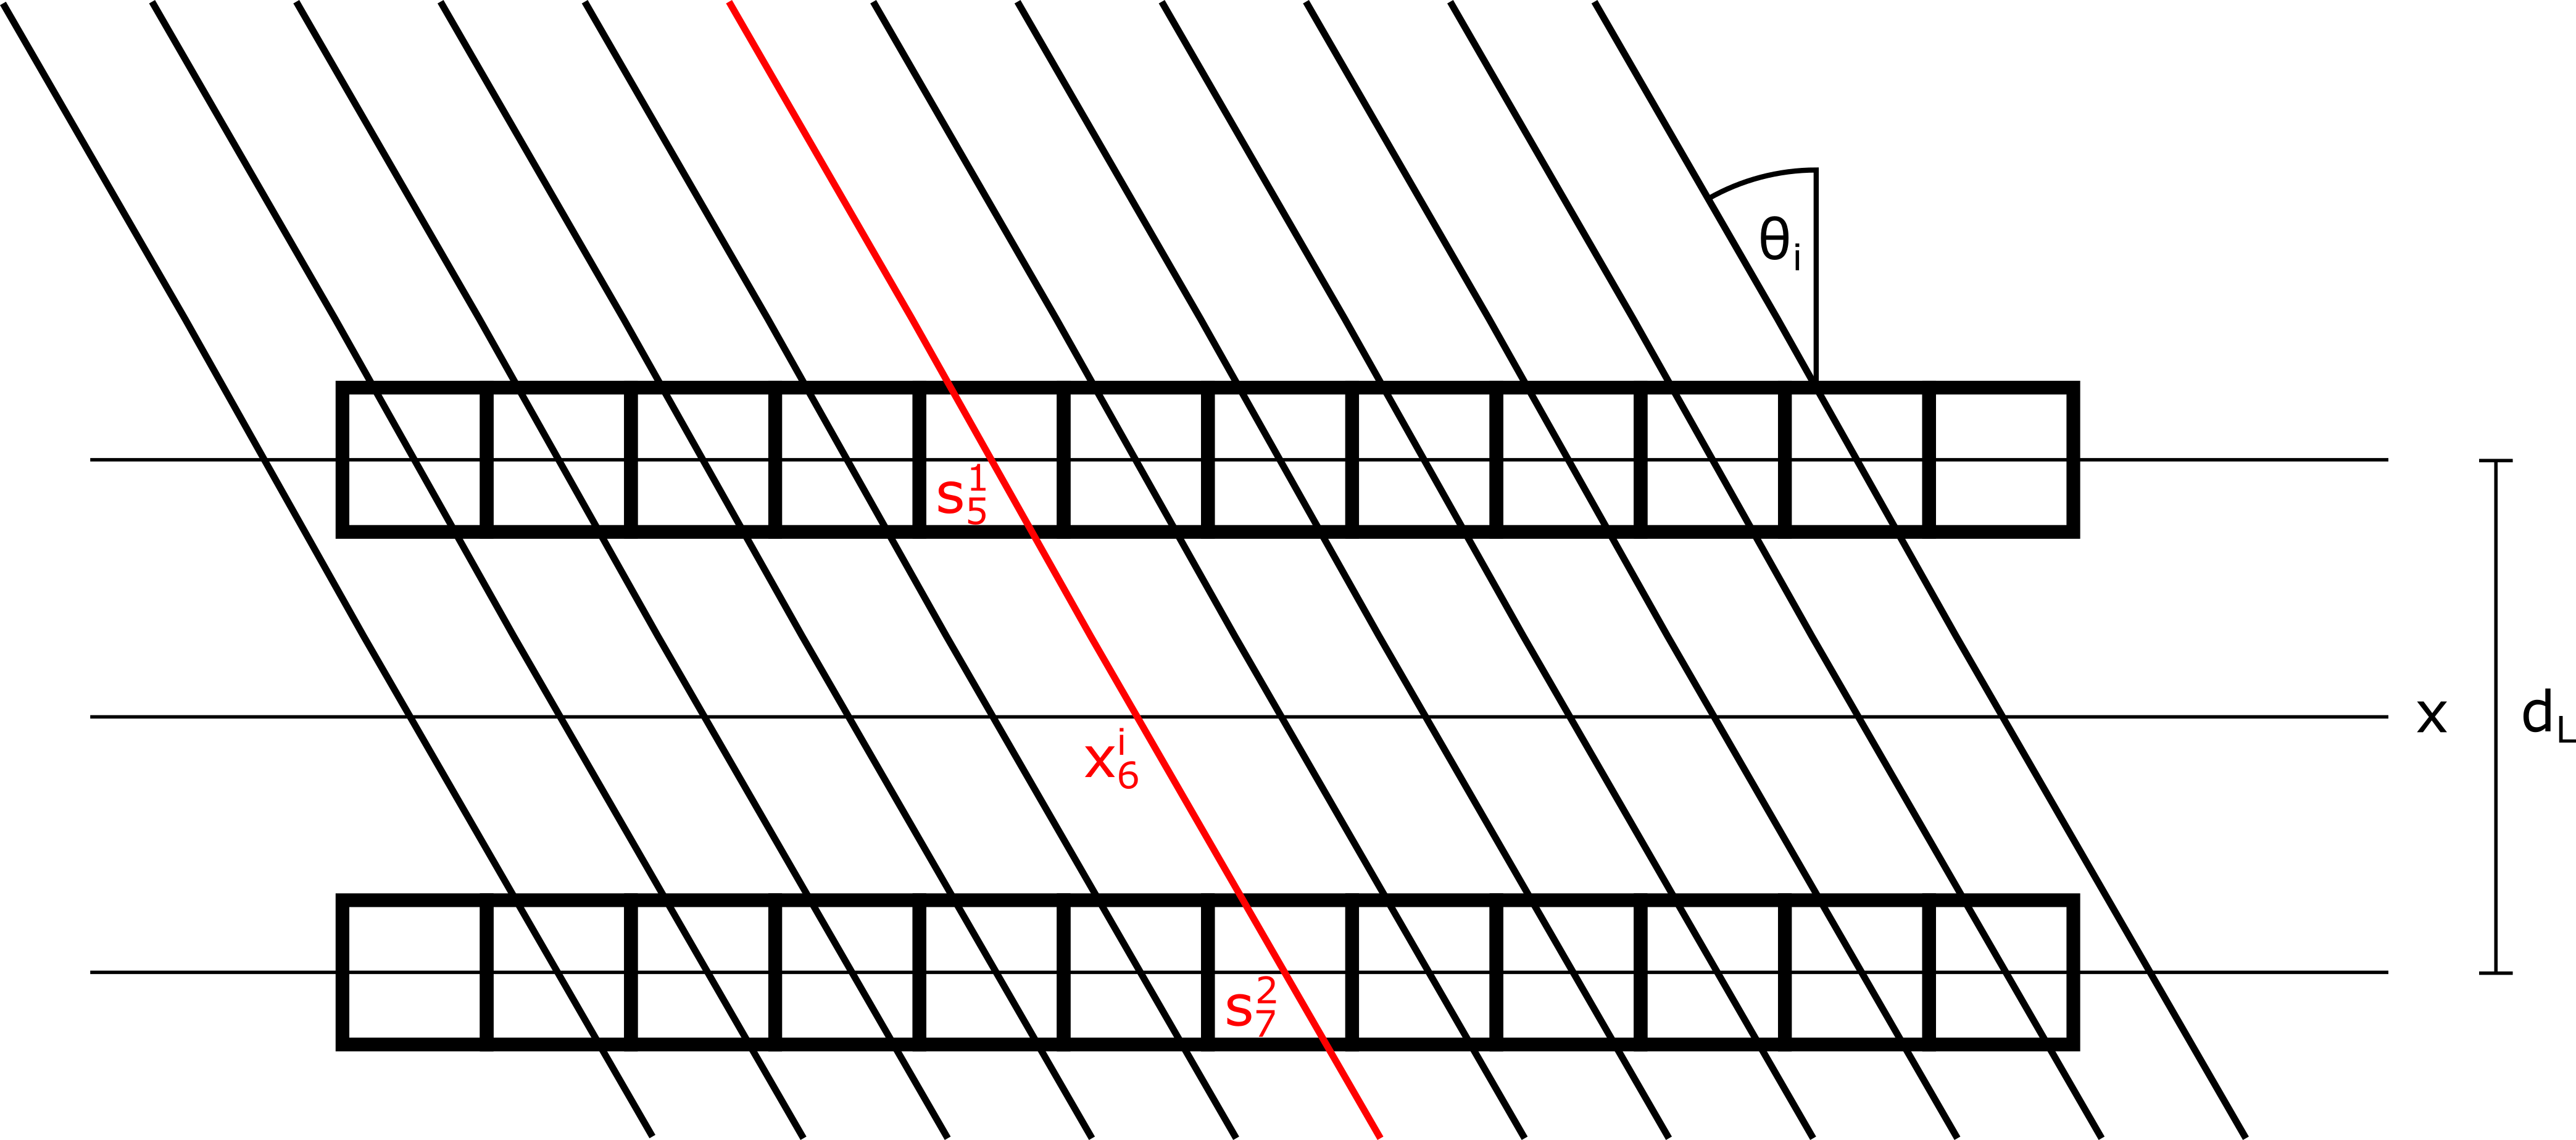
\includegraphics[scale=0.6]{sketches/layers_orthographic_rays.png} 
	\caption{The rays captured by camera $i$ using orthographic projection. All rays from one camera have the same angle $\theta_i$, which is measured relative to the surface normal of the layers. $x_6^i$, $s_5^2$ and $s_7^1$ denote the intersections of the ray with the camera sensor and the layers. $d_L$ is the distance between the layers.}
	\label{fig:orthographic_cameras_layers_sketch}
\end{figure}

Figure \ref{fig:orthographic_cameras_layers_sketch} shows the way we can construct $P$. For each camera we know the angle $\theta_i$. Lets assume we have two layers. We can place the sensor plane between the two layers as shown in figure \ref{fig:orthographic_cameras_layers_sketch}. For a pixels $x^i$ on the sensor plane, we can compute the positions

\begin{align*}
	& s^1 = x^i + \frac{d_L}{2}\tan\left( \theta_i \right) && \text{and} && s^2 = s_1 - d_L \tan\left( \theta_i \right) \text{.}
\end{align*}

Once we have the positions $s^1$ and $s^2$, we compute linear indices $k$ from $\left(i, x^i\right)$, $l_1$ from $\left(s^1, 1\right)$ and $l_2$ from $\left(s^2, 2\right)$. Finally, we set $P\left(k, l_1\right) = 1$ and $P\left(k, l_2\right) = 1$. The extension for 4D-light fields and more layers is straightforward.

Having constructed the matrix $P$ which defines a system of linear equations, I used the iterative  linear least squares solver \emph{lsqlin} in MATLAB to find a solution of equation \ref{eq:core_problem}. This method turns out to be too slow when the matrix is very large. I found another iterative method called The Simultaneous Algebraic Reconstruction Technique (SART) that turns out to be efficient for my problem. It is often used in tomography applications. For the definition and convergence analysis of SART, I refer to \cite{CONV_SART}. 

\section{Moving to light fields of type 1}
The next challenge is to support light fields of type 1, as described in section \ref{sec:lftypes}. The motivation comes from the fact that most (online) light field archives provide datasets of this type. And there is also the plenoptic camera we can produce light fields with. 
\\
The requirements for this setup are the following:

\begin{itemize}
	\item A camera plane of known size/camera positions
	\item The distance from the camera plane to the scene origin: $z$
	\item The distance from the camera plane/center of projection to the sensor plane: $d_s$
	\item The field of view of the cameras
	\item The size and placement of each layer relative to the scene origin
\end{itemize}

I make the assumption that the cameras are pinhole cameras. The disparity of the images is given by $D = x_1 - x_2 = \frac{d_s d_c}{z}$, where $d_c$ is the distance between two cameras.

\subsection{Approach 1: From camera pixels to layer pixels}
My idea for this approach is to go through each pixel for each camera and trace back the ray going through this pixel and the center of projection. Knowing the ray direction, we can compute the intersection with each layer. This gives us pixel correspondences between camera pixel- and layer pixel coordinates. For the valid intersections, we would then add the value 1 in the matrix at the respective index. 
\\
This method does not seem to work. The main problem is that a lot of layer pixels may not be hit by rays for a camera. It heavily depends on the resolution of the cameras and the layers for this method to work. The problem is shown in figure \ref{fig:problem_camera_to_layers}.

\begin{figure}[t]
	\centering
	\begin{subfigure}[t]{0.4\textwidth}
 		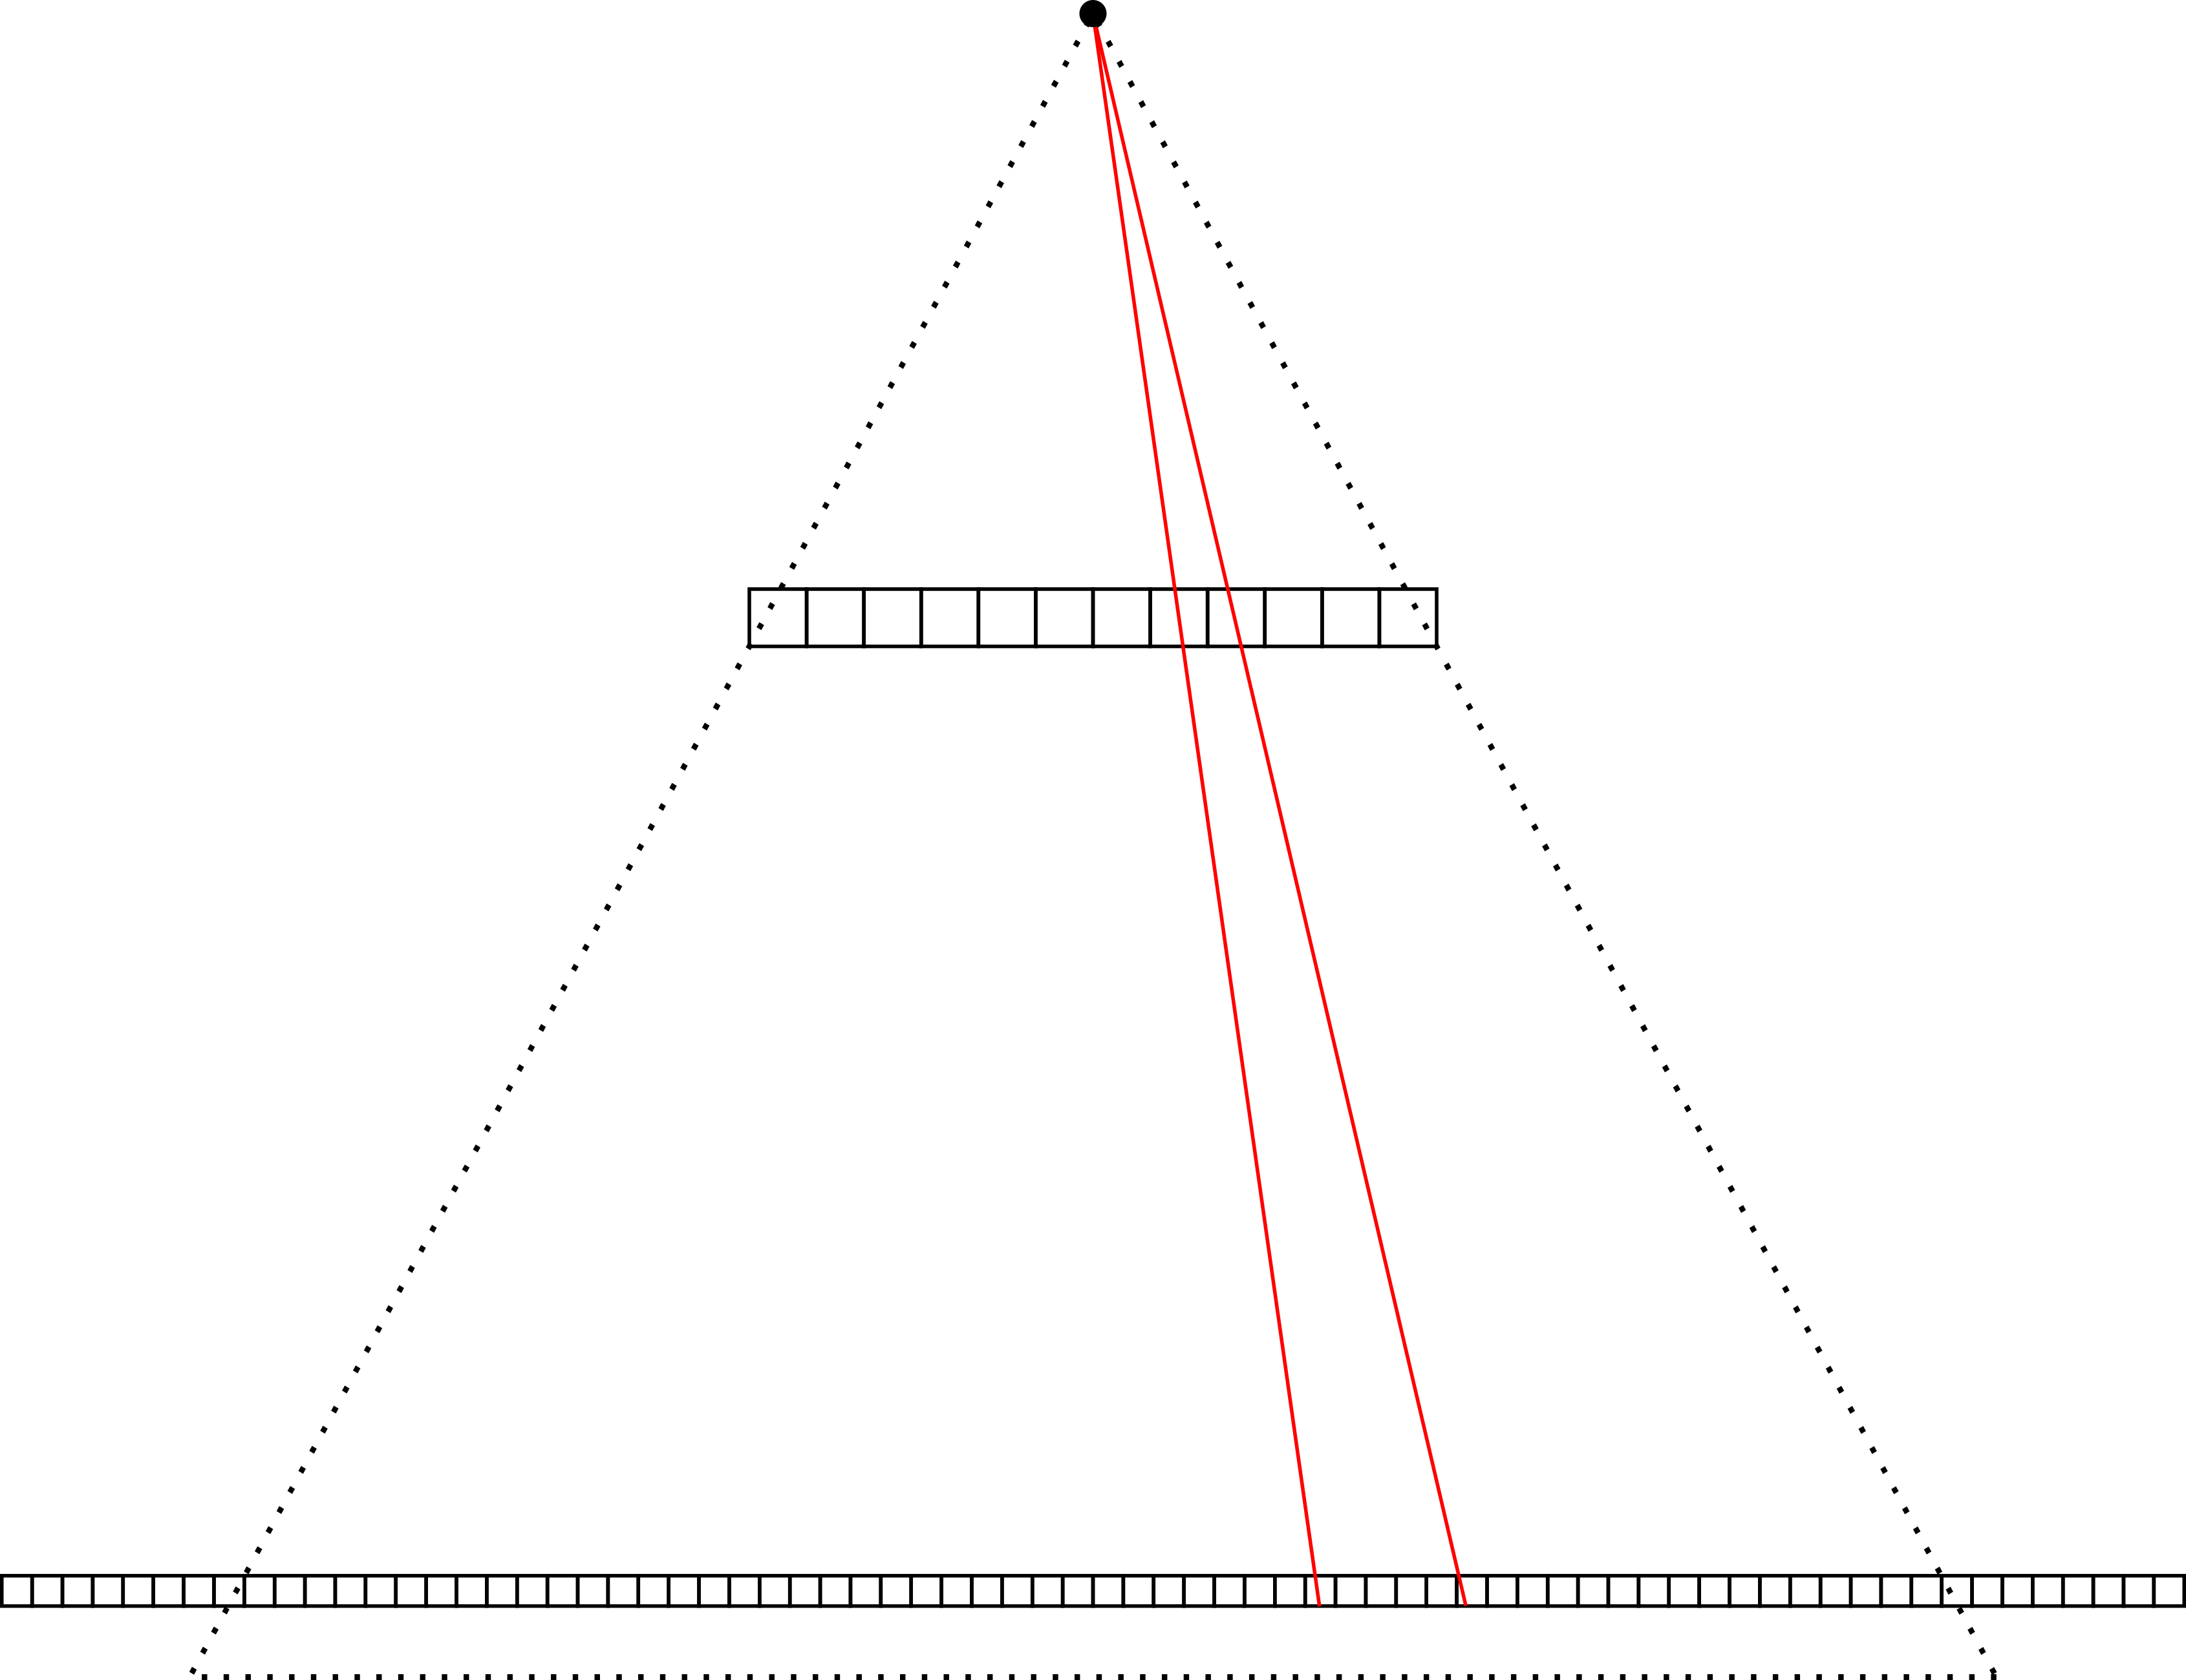
\includegraphics[scale=0.3]{sketches/problem_camera_to_layers.png} 
		\caption{Two rays hitting a cameras sensor in neighbouring pixels. The two rays intersect with the layer pixels, with multiple pixels in between.}
		\label{fig:problem_camera_to_layers}
	\end{subfigure}%
	\qquad
	\begin{subfigure}[t]{0.4\textwidth}
		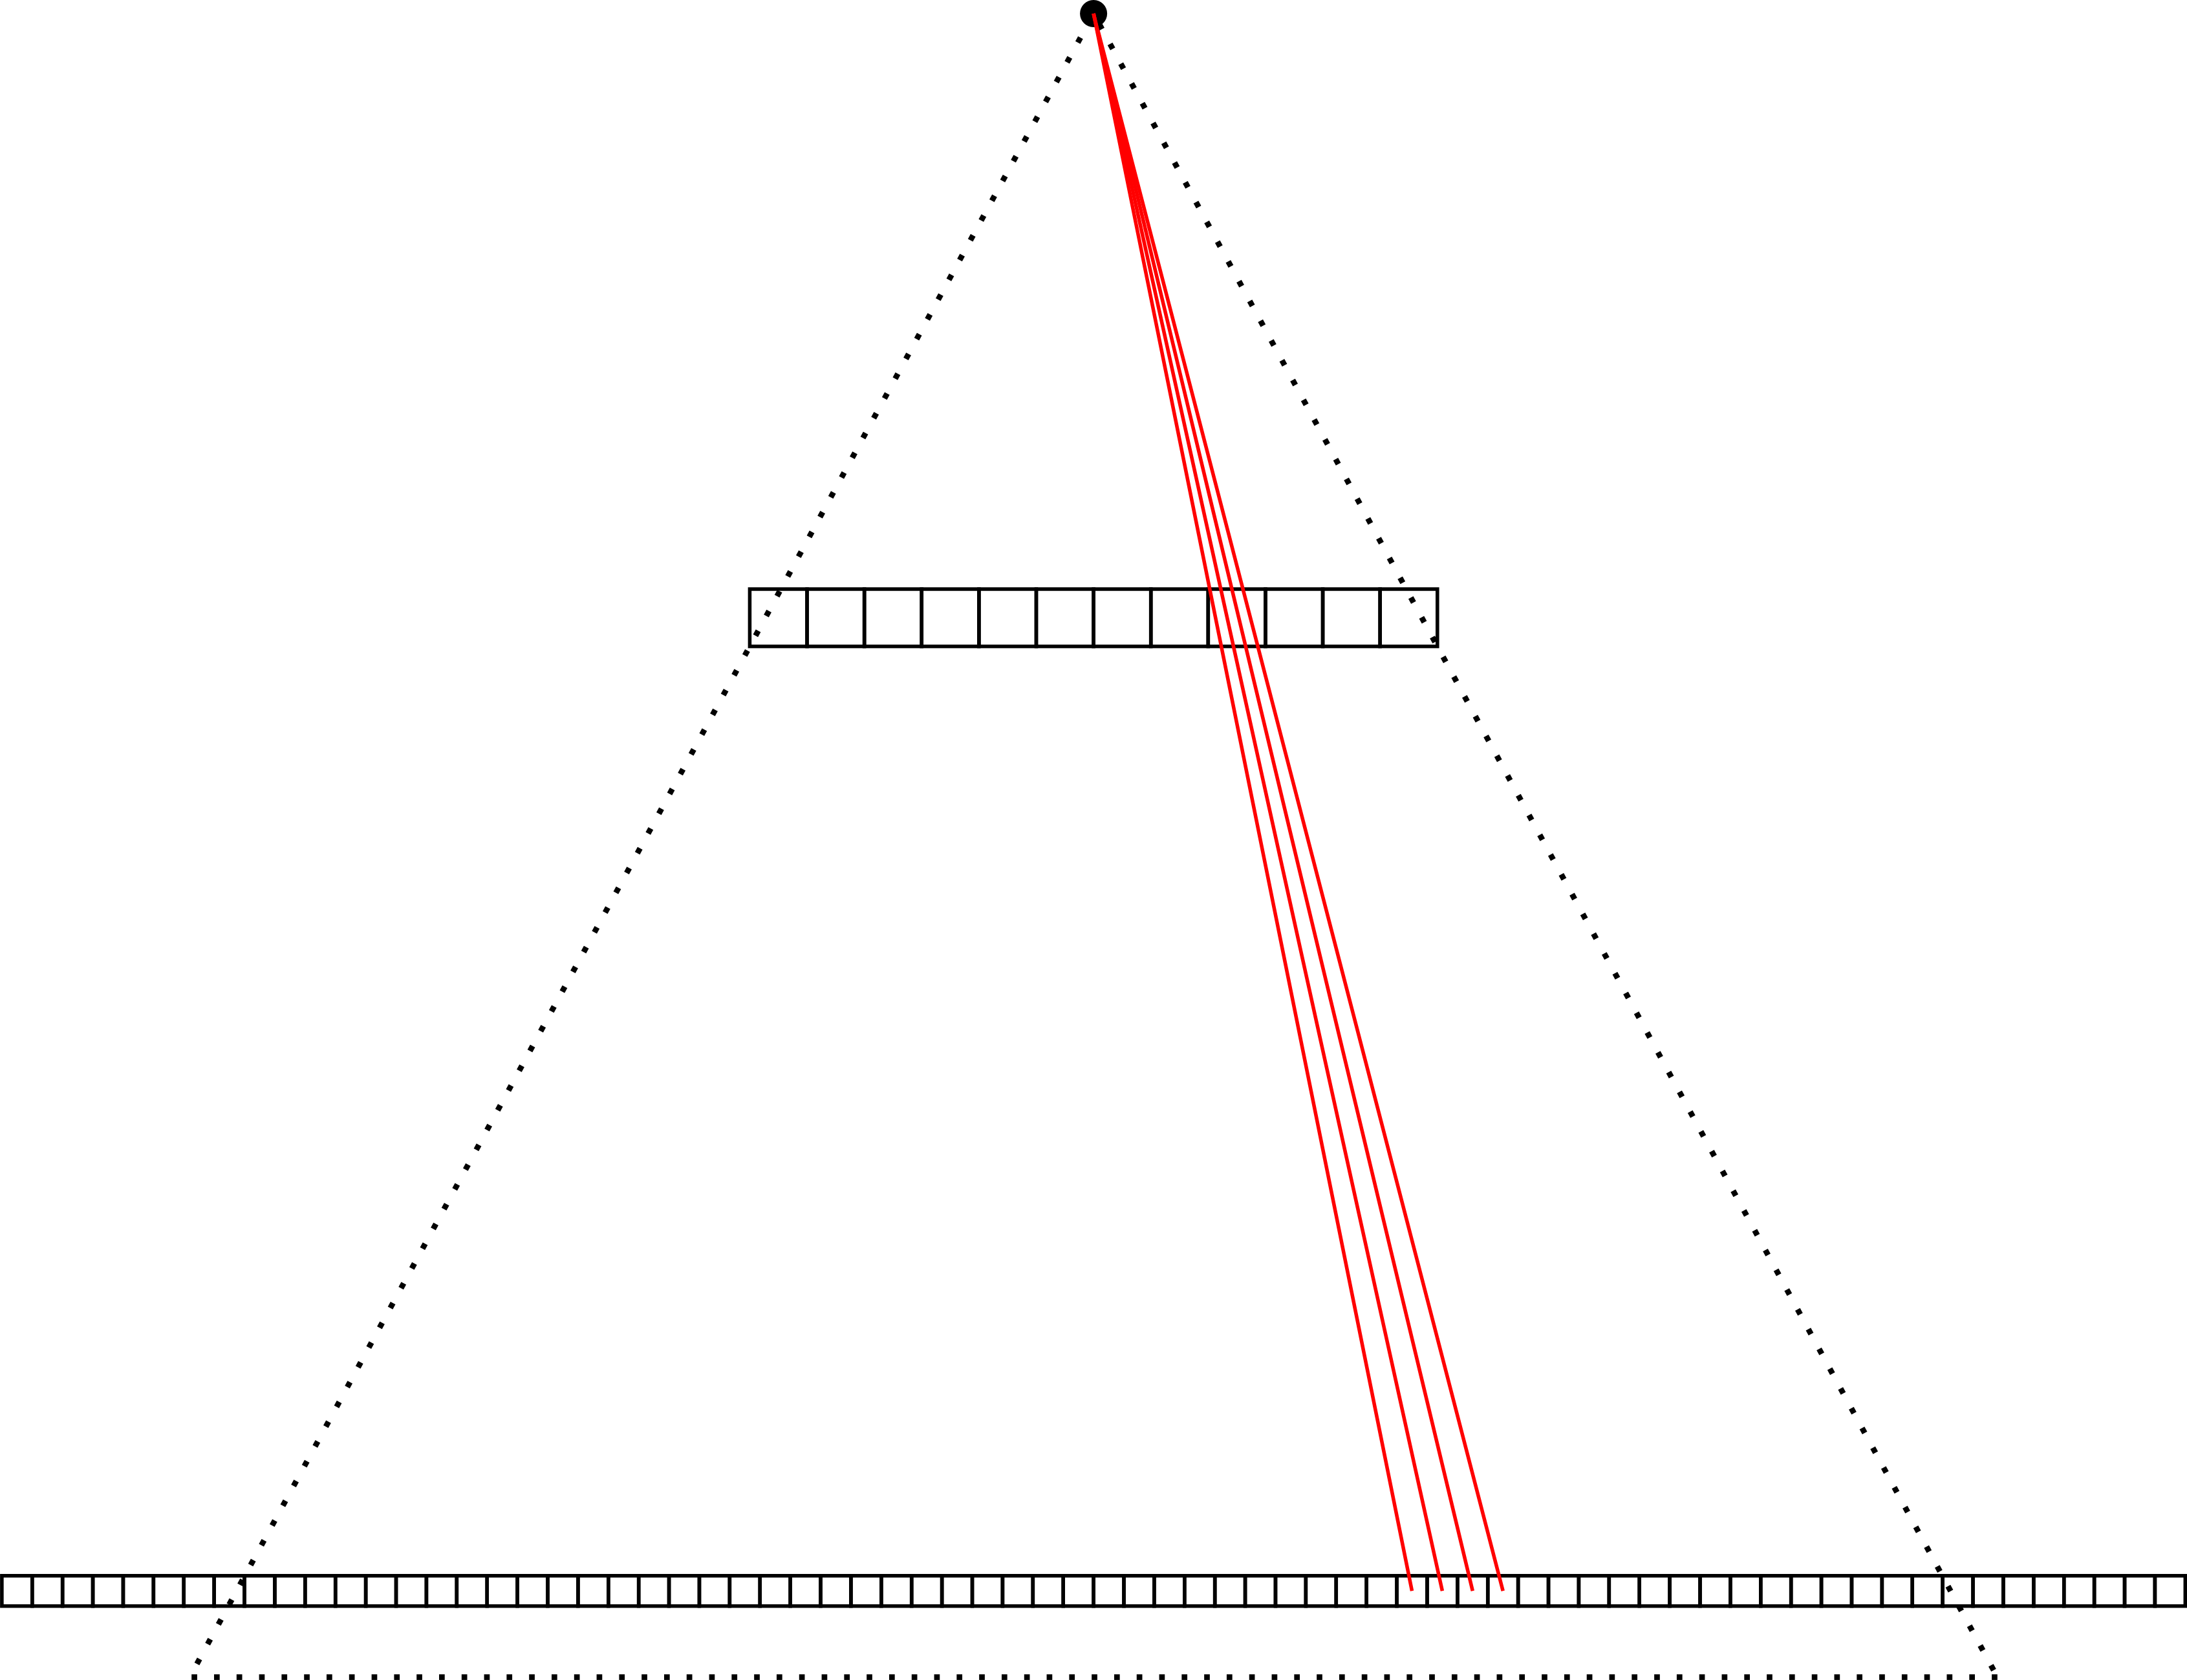
\includegraphics[scale=0.3]{sketches/problem_layers_to_camera_rounding.png}
		\caption{Rays coming from four different layer pixels and hitting the same sensor pixel in the camera.}
		\label{fig:problem_layers_to_camera}
	\end{subfigure}
	\caption{Problems that can arise from different resolution in image- and layer space.}
\end{figure}

\subsection{Approach 2: Converting the light field}
The next idea is to reparametrize the light field $l \left( c_y, c_x, y, x \right)$ to an angular representation $l' \left( \theta_y, \theta_x, v, u \right)$. Here, the number of angles corresponds to the resolution of the camera sensor. The motivation behind this approach is that we can fix 
$\left( \theta_y, \theta_x \right)$ in the latter representation and get an orthogonal view. We would then plug this light field into the old algorithm to solve for the layers.
\\
For the reparametrization, we construct matrices

\begin{align*}
	C_y \left( \theta_y, :, v, : \right) && C_x \left( :, \theta_x, :, u \right) && I_y \left(\theta_y, :, v, : \right) && I_x \left( :, \theta_x, : u \right) 
\end{align*}

of the same dimension as the light field resolution. The ":" represents replication of the matrix in the respective dimension. We use these matrices to obtain a interpolated light field $l' \left( \theta_y, \theta_x, v, u \right)$.
\\\\ TODO: Why didn't it work in the end? 

\subsection{Approach 3: From layer pixels to camera pixels}
This idea is basically the opposite of approach 1. For every layer pixel and for every camera we compute the ray intersection on the sensor plane. The positions $x_j^1$ and $x_j^2$ shown in figure \ref{fig:cameras_layers_sketch} are computed as follows:

\begin{align*}
	& x_j^1 = \left( s_i^1 - u_1 \right) \frac{d_s}{z + d_L} & x_k^2 = \left( s_i^1 - u_2 \right) \frac{d_s}{z + d_L}
\end{align*}

These points will be scaled and rounded to their corresponding pixels. We can then construct the propagation matrix $P$ the same way as in section \ref{sec:first_implementation}.
As demonstrated in figure \ref{fig:problem_layers_to_camera}, it often happens that a patch of layer pixels gets mapped to the same camera pixel due to rounding and thus, one pixel from the camera would contribute to multiple layer pixels. This also results in high column sums of the matrix $P$ from equation \ref{eq:core_problem}.

\begin{figure}[h]
	\centering
	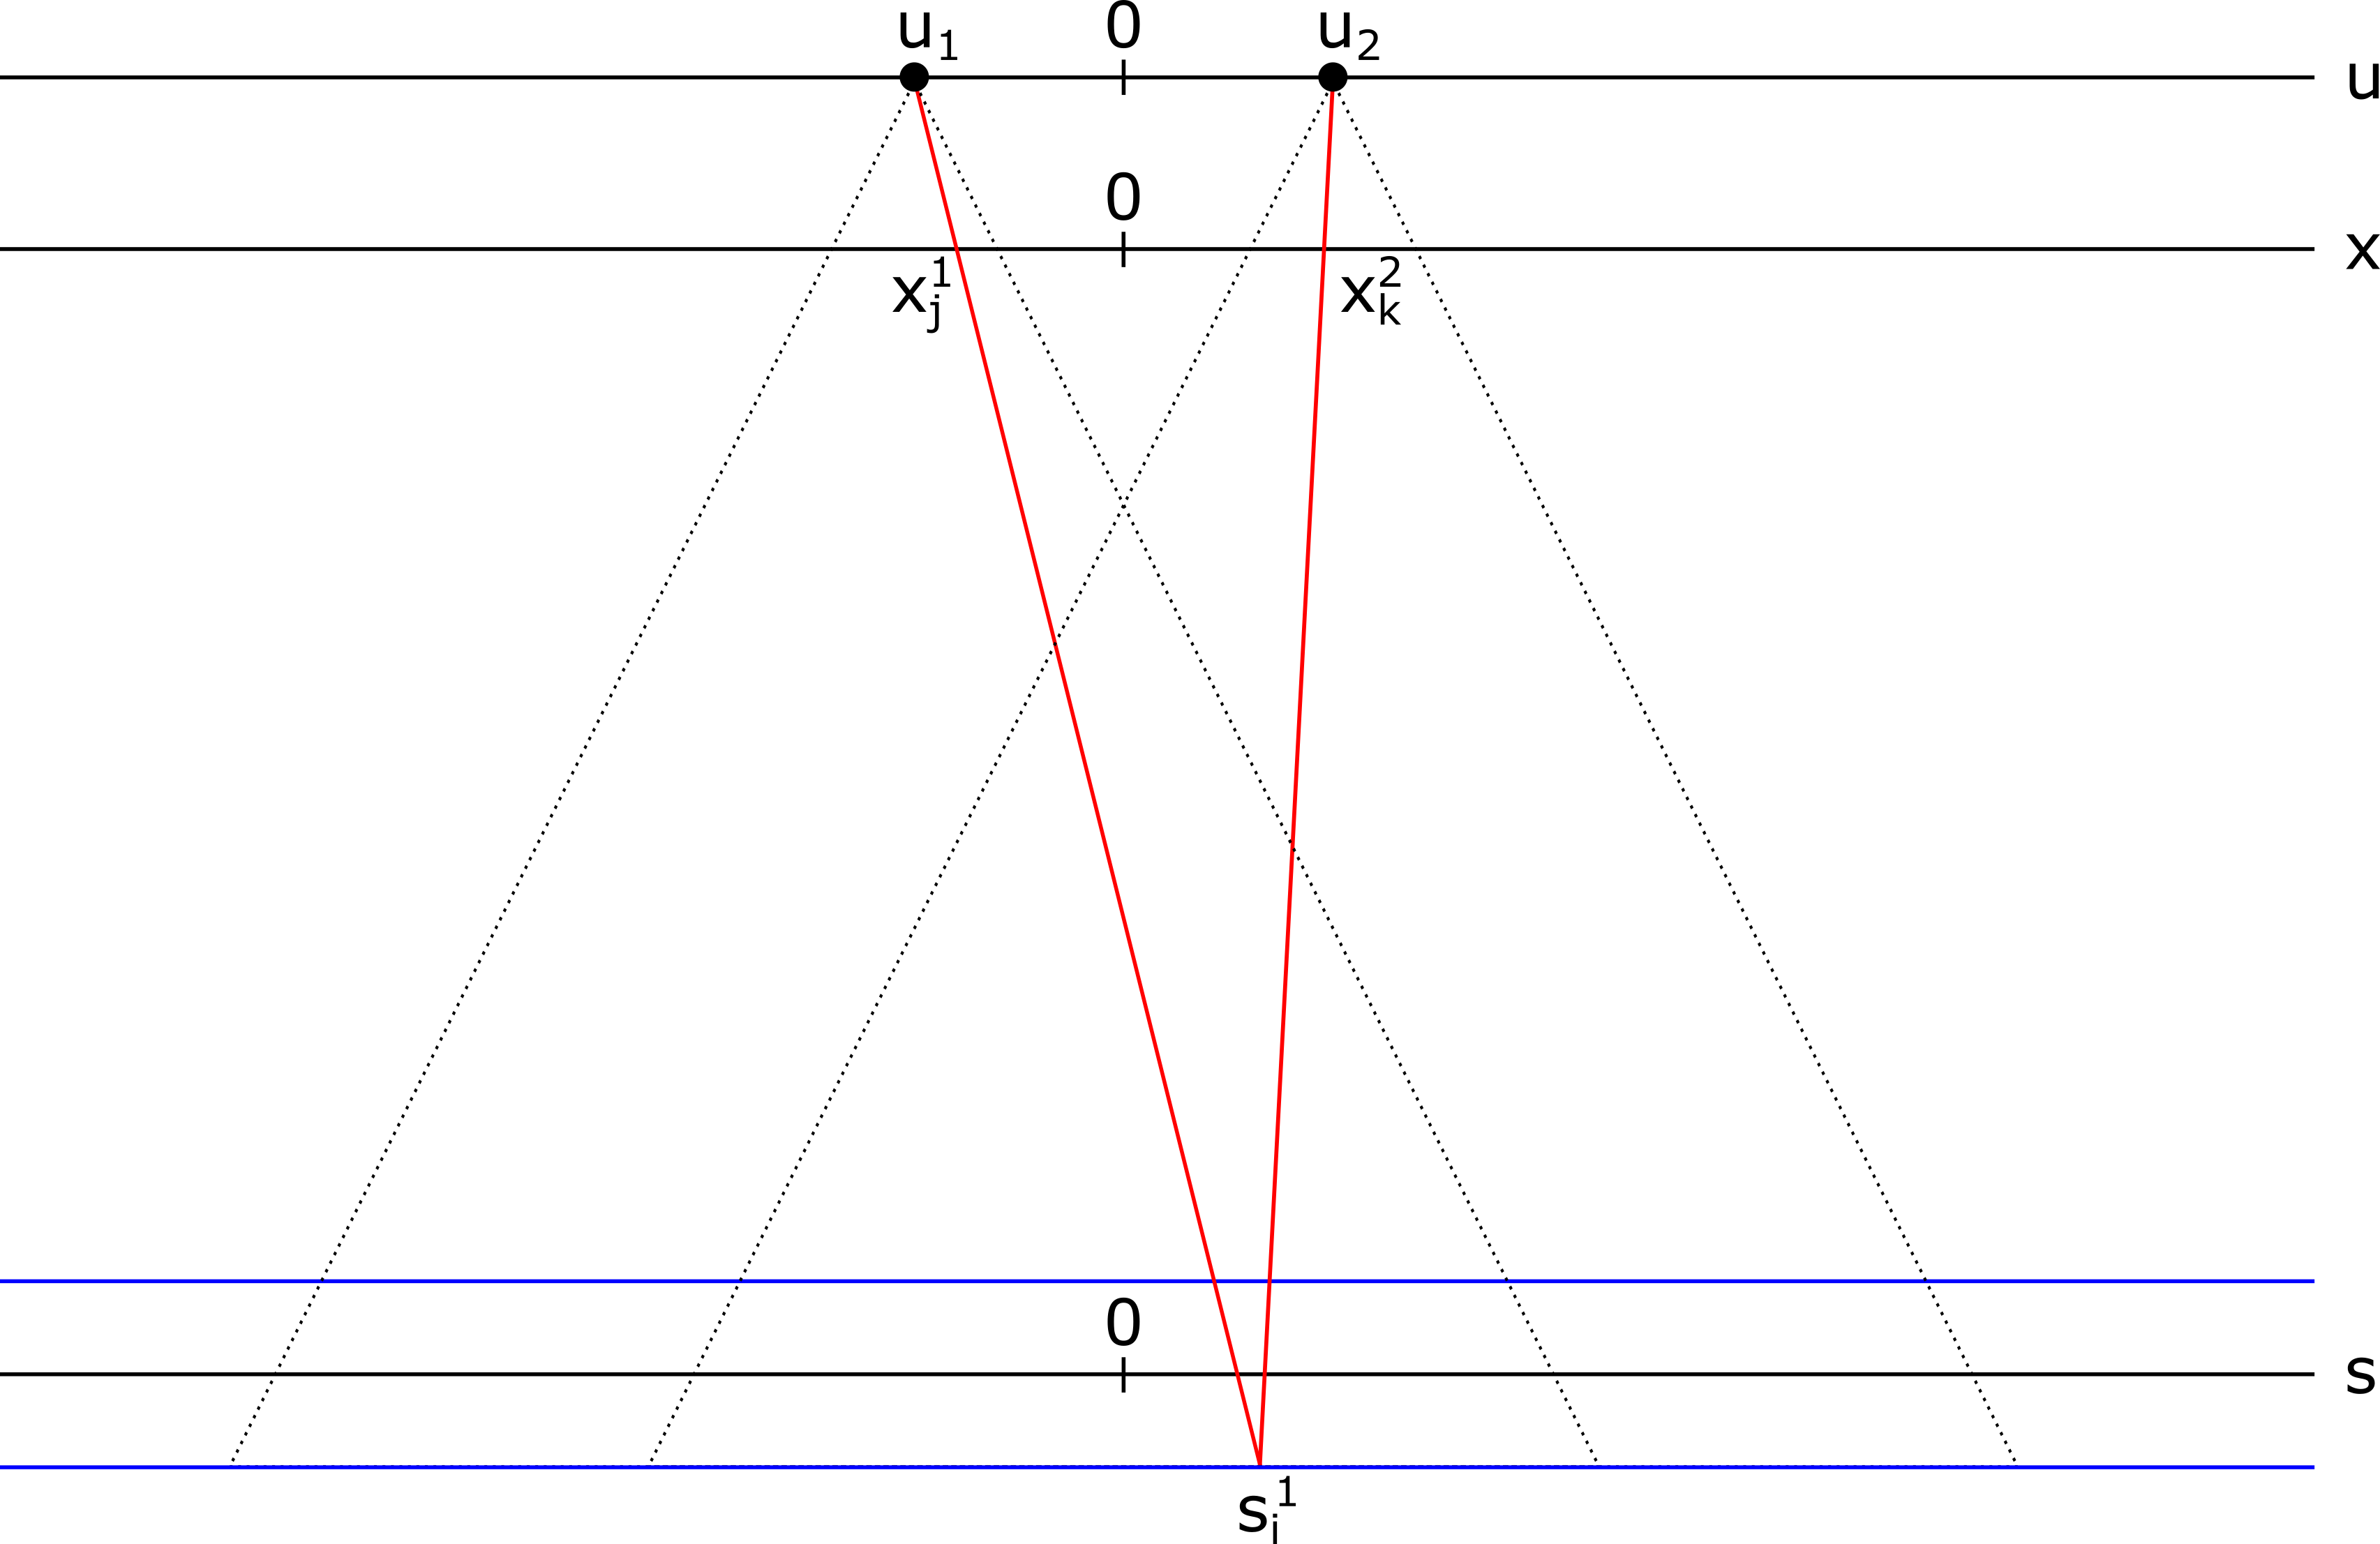
\includegraphics[scale=0.5]{sketches/camera_layers_sketch.png} 
	\caption{Two rays (red) intersecting the first layer (blue) at position $s_i^1$. The rays are captured by different cameras at positions $u_1$ and $u_2$, hitting the camera sensor at locations $x_j^1$ and $x_k^2$. The dotted lines represent the field of view of each camera.}
	\label{fig:cameras_layers_sketch}
\end{figure}

\section{Creating synthetic light fields}
I used light fields from the Heidelberg and Stanford light field archives. In addition, I also rendered synthetic scenes with POV-Ray. The advantage of a synthetic light field is that the cameras can be precisely placed and all the required parameters are known and can be adjusted easily. 

\section{Review of the two implementations}
\subsection{Orthographic projections}
\subsection{Perspective projections}
\newpage
\bibliographystyle{alpha}
\bibliography{lit}

\end{document}


